% \VignetteIndexEntry{TCseq Vignette}
% \VignetteDepends{TCseq}
% \VignetteKeywords{Time course sequencing analysis, Clustering}
% \VignettePackage{TCseq}

\documentclass[a4paper]{article}
\usepackage{a4wide}
\usepackage[utf8]{inputenc}
\usepackage{float}
%~~~~~~~~~~~~~~~~~~~~~~~~~~~~~~~~~~%
\title{TCseq: time course sequencing data analysis}
\author{Mengjun, Lei Gu}
\date{ \today }

%~~~~~~~~~~~~~~~~~~~~~~~~~~~~~~~~~~%
\usepackage{Sweave}
\begin{document}
\Sconcordance{concordance:TCseq.tex:TCseq.Rnw:%
1 15 1 1 0 18 1 1 2 4 0 2 2 1 0 1 1 3 0 2 2 1 0 1 1 12 0 1 2 2 1 1 3 2 %
0 1 1 11 0 1 2 1 0 1 1 11 0 1 2 1 0 1 1 26 0 2 2 4 0 1 2 1 3 2 0 1 2 1 %
0 1 2 1 0 1 1 35 0 2 2 4 0 1 2 3 1 1 2 4 0 2 2 4 0 2 2 1 0 1 1 29 0 1 1 %
12 0 1 2 1 3 2 0 1 1 30 0 1 2 3 1 1 3 5 0 1 2 1 3 5 0 2 2 1 0 1 1 12 0 %
1 2 1 1 1 2 4 0 1 2 3 1 1 2 4 0 1 2 7 1 1 3 5 0 1 2 18 1}

\maketitle

%--------------------------------------------------
The TCseq package provides a unified suite for analysis of different types of time course sequencing data. It can be applied to transcriptome time course data such as RNA-seq as well as epigenome time course data such as ATAC-seq, ChIP-seq. The main focuses of this package are on differential analysis between different time points and temporal pattern analysis and visualization.

Unlike RNA-seq,  the genomic regions of interest of sequencing data like ATAC-seq, ChIP-seq are not pre-defined and are specific to each experimental conditions, which limits the subsequential differential analysis between conditions. For those data type, the TCseq package provides functions to combine and merge conditionally specific genomic regions and generate a reference genomic regions for all conditions. This package then uses the negative binomial generalized linear model implemented in edgeR to provide differential analysis \cite{Robinson}. To capture the temporal patterns of the time course data, the package includes several unsupervised clustering methods to identify and a function to visualize the patterns.

This vignette uses an example ATAC-seq time course data to illustrate how to use the TCseq package.

%--------------------------------------------------
\section{Input data}
The minimal input data for the TCseq are experiment design and reference genomic regions.

\subsection{Generate reference genomic regions}
For RNA-seq, the reference genomic regions are predefined (genes or exons). While for epigenome sequencing data, genomic regions of interest are usually defined as reads enriched regions which are also called peaks. peaks set for a given condition can be identified by peak callers such as MACs and is specific to that condition. The TCseq package provides a function to read in a set of peak set file in BED format, combines these files in to a single data frame, merges overlapping regions according use defined criteria and takes the largest bound as the reference region for all the overlapping regions. The merge criteria can be either absolute overlapping bases or overlapping ration (absolute overlapping bases divide mininum length of the regions to be merged).

If a set of BED files are availble under certain directory, say dir.peaks, the file names of the BED files to be merged have common substring "narrowpeaks", then the reference genomic regions can be generated by:
\begin{Schunk}
\begin{Sinput}
> library(TCseq)
\end{Sinput}
\end{Schunk}

\begin{Schunk}
\begin{Sinput}
> dir <- dir.peaks
> gf <- peakreference(dir = dir, pattern = "narrowpeaks")
\end{Sinput}
\end{Schunk}
The resulting data frame have four columns as follows:
\begin{Schunk}
\begin{Sinput}
> data("genomicIntervals")
> head(genomicIntervals)
\end{Sinput}
\begin{Soutput}
    chr    start      end    id
11 chr1  6453992  6454731 peak1
18 chr1  7823890  7824372 peak2
19 chr1  8029820  8030138 peak3
20 chr1  8030317  8030627 peak4
39 chr1 10880000 10880701 peak5
41 chr1 13154468 13154786 peak6
\end{Soutput}
\end{Schunk}

\subsection{Create a TCA object}
The TCseq uses an S4 class TCA to store all input data for subsequential analysis. When read counts table is not available, only experiment design and reference genomic regions as data frames are required to create a TCA object, TCseq also provides a function to generate counts table, to use the function, file names of BAM files for each sample/library have to be provided in the data frame of experiment design:
\begin{Schunk}
\begin{Sinput}
> # Experiment design
> data("experiment_BAMfile")
> head(experiment_BAMfile)
\end{Sinput}
\begin{Soutput}
  sampleid timepoint group       bamfile
1       s1        0h     1   rep1_0h.bam
2       s2       24h     2  rep1_24h.bam
3       s3       40h     3  rep1_40h.bam
4       s4       56h     4  rep1_56h.bam
5       s5       72h     5  rep1_72h.bam
6       s6      120h     6 rep1_120h.bam
\end{Soutput}
\begin{Sinput}
> #reference genomic regions
> data("genomicIntervals")
> head(genomicIntervals)
\end{Sinput}
\begin{Soutput}
    chr    start      end    id
11 chr1  6453992  6454731 peak1
18 chr1  7823890  7824372 peak2
19 chr1  8029820  8030138 peak3
20 chr1  8030317  8030627 peak4
39 chr1 10880000 10880701 peak5
41 chr1 13154468 13154786 peak6
\end{Soutput}
\begin{Sinput}
> # create a TCA object
> tca <- TCA(design = experiment_BAMfile, genomicFeature = genomicIntervals)
> tca
\end{Sinput}
\begin{Soutput}
An object of class "TCA"
@design
  sampleid timepoint group      bamfile
1       s1        0h     1  rep1_0h.bam
2       s2       24h     2 rep1_24h.bam
3       s3       40h     3 rep1_40h.bam
4       s4       56h     4 rep1_56h.bam
5       s5       72h     5 rep1_72h.bam
7 more rows ...

@genomicFeature
    chr    start      end    id
11 chr1  6453992  6454731 peak1
18 chr1  7823890  7824372 peak2
19 chr1  8029820  8030138 peak3
20 chr1  8030317  8030627 peak4
39 chr1 10880000 10880701 peak5
2746 more rows ...

@clusterRes
An object of class "clust"
\end{Soutput}
\end{Schunk}
The count table then can be created (suppose the BAM files are store in the directory dir.BAM):
\begin{Schunk}
\begin{Sinput}
> tca <- countReads(tca, dir = dir.BAM)
\end{Sinput}
\end{Schunk}
When the counts table is available, BAM file information is not mandatory in the experiment design. Counts table can be provides when creating a TCA object:
\begin{Schunk}
\begin{Sinput}
> #Experiment design without BAM file information
> data("experiment")
> #Counts table
> data("countsTable")
> tca <- TCA(design = experiment, genomicFeature = genomicIntervals,
+            counts = countsTable)
> tca
\end{Sinput}
\begin{Soutput}
An object of class "TCA"
@design
  sampleid timepoint group
1       s1        0h     1
2       s2       24h     2
3       s3       40h     3
4       s4       56h     4
5       s5       72h     5
7 more rows ...

@counts
       s1  s2  s3  s4  s5  s6  s7  s8  s9 s10 s11 s12
peak1 344 243 169  70  57  20 298 199 135  63  54  34
peak2  72 114  91  93 133 164  55  71  93 116 150 191
peak3  28  50 109 115  94 109  60  89  75 129  85 101
peak4  28  49 110 113 103 108  59  89  77 131  83 104
peak5 464 344 280 154 108  33 444 255 259 155  97  32
2746 more rows ...

@genomicFeature
    chr    start      end    id
11 chr1  6453992  6454731 peak1
18 chr1  7823890  7824372 peak2
19 chr1  8029820  8030138 peak3
20 chr1  8030317  8030627 peak4
39 chr1 10880000 10880701 peak5
2746 more rows ...

@clusterRes
An object of class "clust"
\end{Soutput}
\end{Schunk}
The counts table can also be assigned to an existing TCA object:
\begin{Schunk}
\begin{Sinput}
> counts(tca) <- countsTable
\end{Sinput}
\end{Schunk}
The TCA object with experiment design, read counts, reference genomic regions can be used for following differential analysis.
%--------------------------------------------------
\section{Differential Analysis}
The differetial event is detected by using the generalized linear model (GLM) methods \cite{McCarthy} implemented in edgeR package.
\begin{Schunk}
\begin{Sinput}
> tca <- DBanalysis(tca)
\end{Sinput}
\end{Schunk}
Low quality genomic regions (read counts are low for all the time points) can also be filtered out. The following step only keeps genomic regions with two or more more samples that have read counts more than 10.
\begin{Schunk}
\begin{Sinput}
> tca <- DBanalysis(tca, filter.type = "raw", filter.value = 10, samplePassfilter = 2)
\end{Sinput}
\end{Schunk}
Differential analysis results between given timepoints can be extracted by:
\begin{Schunk}
\begin{Sinput}
> DBres <- DBresult(tca, group1 = "0h", group2 = c("24h","40h","72h"))
> str(DBres, strict.width =  "cut")
\end{Sinput}
\begin{Soutput}
List of 3
 $ 24hvs0h:'data.frame':	2751 obs. of  7 variables:
  ..$ logFC : num [1:2751] -0.232 0.836 0.984 0.992 -0.304 ...
  ..$ PValue: num [1:2751] 0.158202 0.000135 0.000846 0.000783 0.03408 ...
  ..$ paj   : num [1:2751] 0.37427 0.00382 0.01331 0.01253 0.14626 ...
  ..$ chr   : Factor w/ 21 levels "chr1","chr10",..: 1 1 1 1 1 1 1 1 1 1 ...
  ..$ start : int [1:2751] 6453992 7823890 8029820 8030317 10880000 13154468 1..
  ..$ end   : int [1:2751] 6454731 7824372 8030138 8030627 10880701 13154786 1..
  ..$ id    : chr [1:2751] "peak1" "peak2" "peak3" "peak4" ...
 $ 40hvs0h:'data.frame':	2751 obs. of  7 variables:
  ..$ logFC : num [1:2751] -0.3885 1.2312 1.7198 1.7607 -0.0619 ...
  ..$ PValue: num [1:2751] 2.28e-02 1.86e-08 2.46e-09 9.96e-10 6.69e-01 ...
  ..$ paj   : num [1:2751] 4.12e-02 1.53e-07 2.41e-08 1.09e-08 7.21e-01 ...
  ..$ chr   : Factor w/ 21 levels "chr1","chr10",..: 1 1 1 1 1 1 1 1 1 1 ...
  ..$ start : int [1:2751] 6453992 7823890 8029820 8030317 10880000 13154468 1..
  ..$ end   : int [1:2751] 6454731 7824372 8030138 8030627 10880701 13154786 1..
  ..$ id    : chr [1:2751] "peak1" "peak2" "peak3" "peak4" ...
 $ 72hvs0h:'data.frame':	2751 obs. of  7 variables:
  ..$ logFC : num [1:2751] -1.189 2.499 2.337 2.408 -0.809 ...
  ..$ PValue: num [1:2751] 1.90e-09 2.71e-33 7.69e-16 8.74e-17 7.38e-07 ...
  ..$ paj   : num [1:2751] 3.20e-09 1.56e-32 1.84e-15 2.22e-16 1.07e-06 ...
  ..$ chr   : Factor w/ 21 levels "chr1","chr10",..: 1 1 1 1 1 1 1 1 1 1 ...
  ..$ start : int [1:2751] 6453992 7823890 8029820 8030317 10880000 13154468 1..
  ..$ end   : int [1:2751] 6454731 7824372 8030138 8030627 10880701 13154786 1..
  ..$ id    : chr [1:2751] "peak1" "peak2" "peak3" "peak4" ...
\end{Soutput}
\begin{Sinput}
> head(DBres$`24hvs0h`)
\end{Sinput}
\begin{Soutput}
           logFC       PValue         paj  chr    start      end    id
peak1 -0.2322614 0.1582019050 0.374266709 chr1  6453992  6454731 peak1
peak2  0.8357387 0.0001349142 0.003818077 chr1  7823890  7824372 peak2
peak3  0.9840522 0.0008463822 0.013305128 chr1  8029820  8030138 peak3
peak4  0.9915395 0.0007834517 0.012530672 chr1  8030317  8030627 peak4
peak5 -0.3043052 0.0340797349 0.146261078 chr1 10880000 10880701 peak5
peak6 -0.1883967 0.4047199035 0.655933437 chr1 13154468 13154786 peak6
\end{Soutput}
\end{Schunk}
Significant differential events (log2-fold > 2 or log2-fold < -2, adjusted p-value < 0.05) can be further extracted by:
\begin{Schunk}
\begin{Sinput}
> DBres.sig <- DBresult.filter(DBres, pvalue = "paj", pvalue.threshold = 0.05,
+                              abs.fold = 2, direction = "both")
> str(DBres.sig, strict.width =  "cut")
\end{Sinput}
\begin{Soutput}
List of 3
 $ 24hvs0h:'data.frame':	8 obs. of  7 variables:
  ..$ logFC : num [1:8] 2.54 2.27 2.16 2.74 2.01 ...
  ..$ PValue: num [1:8] 3.77e-11 1.64e-07 7.38e-20 1.15e-06 5.97e-04 ...
  ..$ paj   : num [1:8] 3.46e-08 3.01e-05 2.03e-16 1.13e-04 1.04e-02 ...
  ..$ chr   : Factor w/ 21 levels "chr1","chr10",..: 6 11 13 16 16 17 19 19
  ..$ start : int [1:8] 60749878 28531781 105257039 26014394 53996710 11344347..
  ..$ end   : int [1:8] 60750276 28532149 105257992 26014703 53996920 11344388..
  ..$ id    : chr [1:8] "peak767" "peak1298" "peak1667" "peak2103" ...
 $ 40hvs0h:'data.frame':	79 obs. of  7 variables:
  ..$ logFC : num [1:79] 2.06 2.05 2 2.78 2.38 ...
  ..$ PValue: num [1:79] 3.64e-15 1.34e-12 1.76e-05 1.37e-19 7.46e-18 ...
  ..$ paj   : num [1:79] 1.07e-13 2.69e-11 7.05e-05 7.83e-18 3.42e-16 ...
  ..$ chr   : Factor w/ 21 levels "chr1","chr10",..: 1 1 1 2 2 3 3 3 3 3 ...
  ..$ start : int [1:79] 39578519 72196186 125343128 3697414 67047710 8709536 ..
  ..$ end   : int [1:79] 39578881 72196559 125343477 3697921 67048151 8709931 ..
  ..$ id    : chr [1:79] "peak28" "peak58" "peak102" "peak189" ...
 $ 72hvs0h:'data.frame':	979 obs. of  7 variables:
  ..$ logFC : num [1:979] 2.5 2.34 2.41 2.4 3.11 ...
  ..$ PValue: num [1:979] 2.71e-33 7.69e-16 8.74e-17 9.62e-14 1.47e-33 ...
  ..$ paj   : num [1:979] 1.56e-32 1.84e-15 2.22e-16 2.07e-13 8.62e-33 ...
  ..$ chr   : Factor w/ 21 levels "chr1","chr10",..: 1 1 1 1 1 1 1 1 1 1 ...
  ..$ start : int [1:979] 7823890 8029820 8030317 33502880 37561826 39578519 5..
  ..$ end   : int [1:979] 7824372 8030138 8030627 33503237 37562318 39578881 5..
  ..$ id    : chr [1:979] "peak2" "peak3" "peak4" "peak14" ...
\end{Soutput}
\end{Schunk}
%--------------------------------------------------
\section{Temporal pattern analysis}
\subsection{Construct time course table}
To detect temporal patterns of the time course sequencing data, the TCseq package uses unsupervised clustering methods. First, a time course table is created for clustering analysis. The rows of the time course table are genomic regions, and the columns are time points, the values can be chosen from normalized read counts or logFC of all time points compared to the initial time point. Such table can be created as follows:
\begin{Schunk}
\begin{Sinput}
> # values are logFC
> tca <- timecourseTable(tca, value = "FC", norm.method = "rpkm", filter = TRUE)
\end{Sinput}
\end{Schunk}
or
\begin{Schunk}
\begin{Sinput}
> # values are normalized read counts
> tca <- timecourseTable(tca, value = "expression", norm.method = "rpkm", filter = TRUE)
\end{Sinput}
\end{Schunk}
When the "filter" parameter is set to be TRUE, the time course table will filter out all genomic regions with no significant changes between any two time points. The table can be accessed by:
\begin{Schunk}
\begin{Sinput}
> t <- tcTable(tca)
> head(t)
\end{Sinput}
\begin{Soutput}
                0h       24h       40h      56h      72h      120h
peak767  20.602720 122.53103 215.45264 457.1920 679.5218 1001.9488
peak1298 19.677065 100.91683 297.78073 668.2194 779.7382  250.8255
peak1667 31.716975 142.26128 387.47324 666.9718 800.7809  634.0918
peak2103 46.542402 313.97751 362.09517 857.1818 979.5473  976.4725
peak2129 17.421163  72.14858 237.62324 490.9435 781.7799  448.2977
peak2369  2.523052  22.77127  65.60794 189.1049 388.9364 1090.6255
\end{Soutput}
\end{Schunk}
\subsection{Clustering analysis}
Two types of clustering algorithms are included in the package: hard clustering (hierachical, pam, kmeans) and soft clustering (fuzzy cmeans \cite{Futschik}). The temporal patterns are analyzed using the following function:
\begin{Schunk}
\begin{Sinput}
> tca <- timeclust(tca, algo = "cm", k = 6, standardize = TRUE)
\end{Sinput}
\end{Schunk}
Instead of absolute value of different time series, one might only focus on the change patterns and expect time series with similar pattern to be cluster in same group. In this case, "standardize" parameter gives an option to perform z-score transformation on the data to be clustered, which reduces the noises introduced by the difference in the absolute values.

\subsection{Visualize the clustering results}
The clustering results can be visualized as follows:
\begin{Schunk}
\begin{Sinput}
> p <- timeclustplot(tca, value = "z-score(PRKM)", cols = 3)
\end{Sinput}
\end{Schunk}

\begin{figure}[H]
\centering
        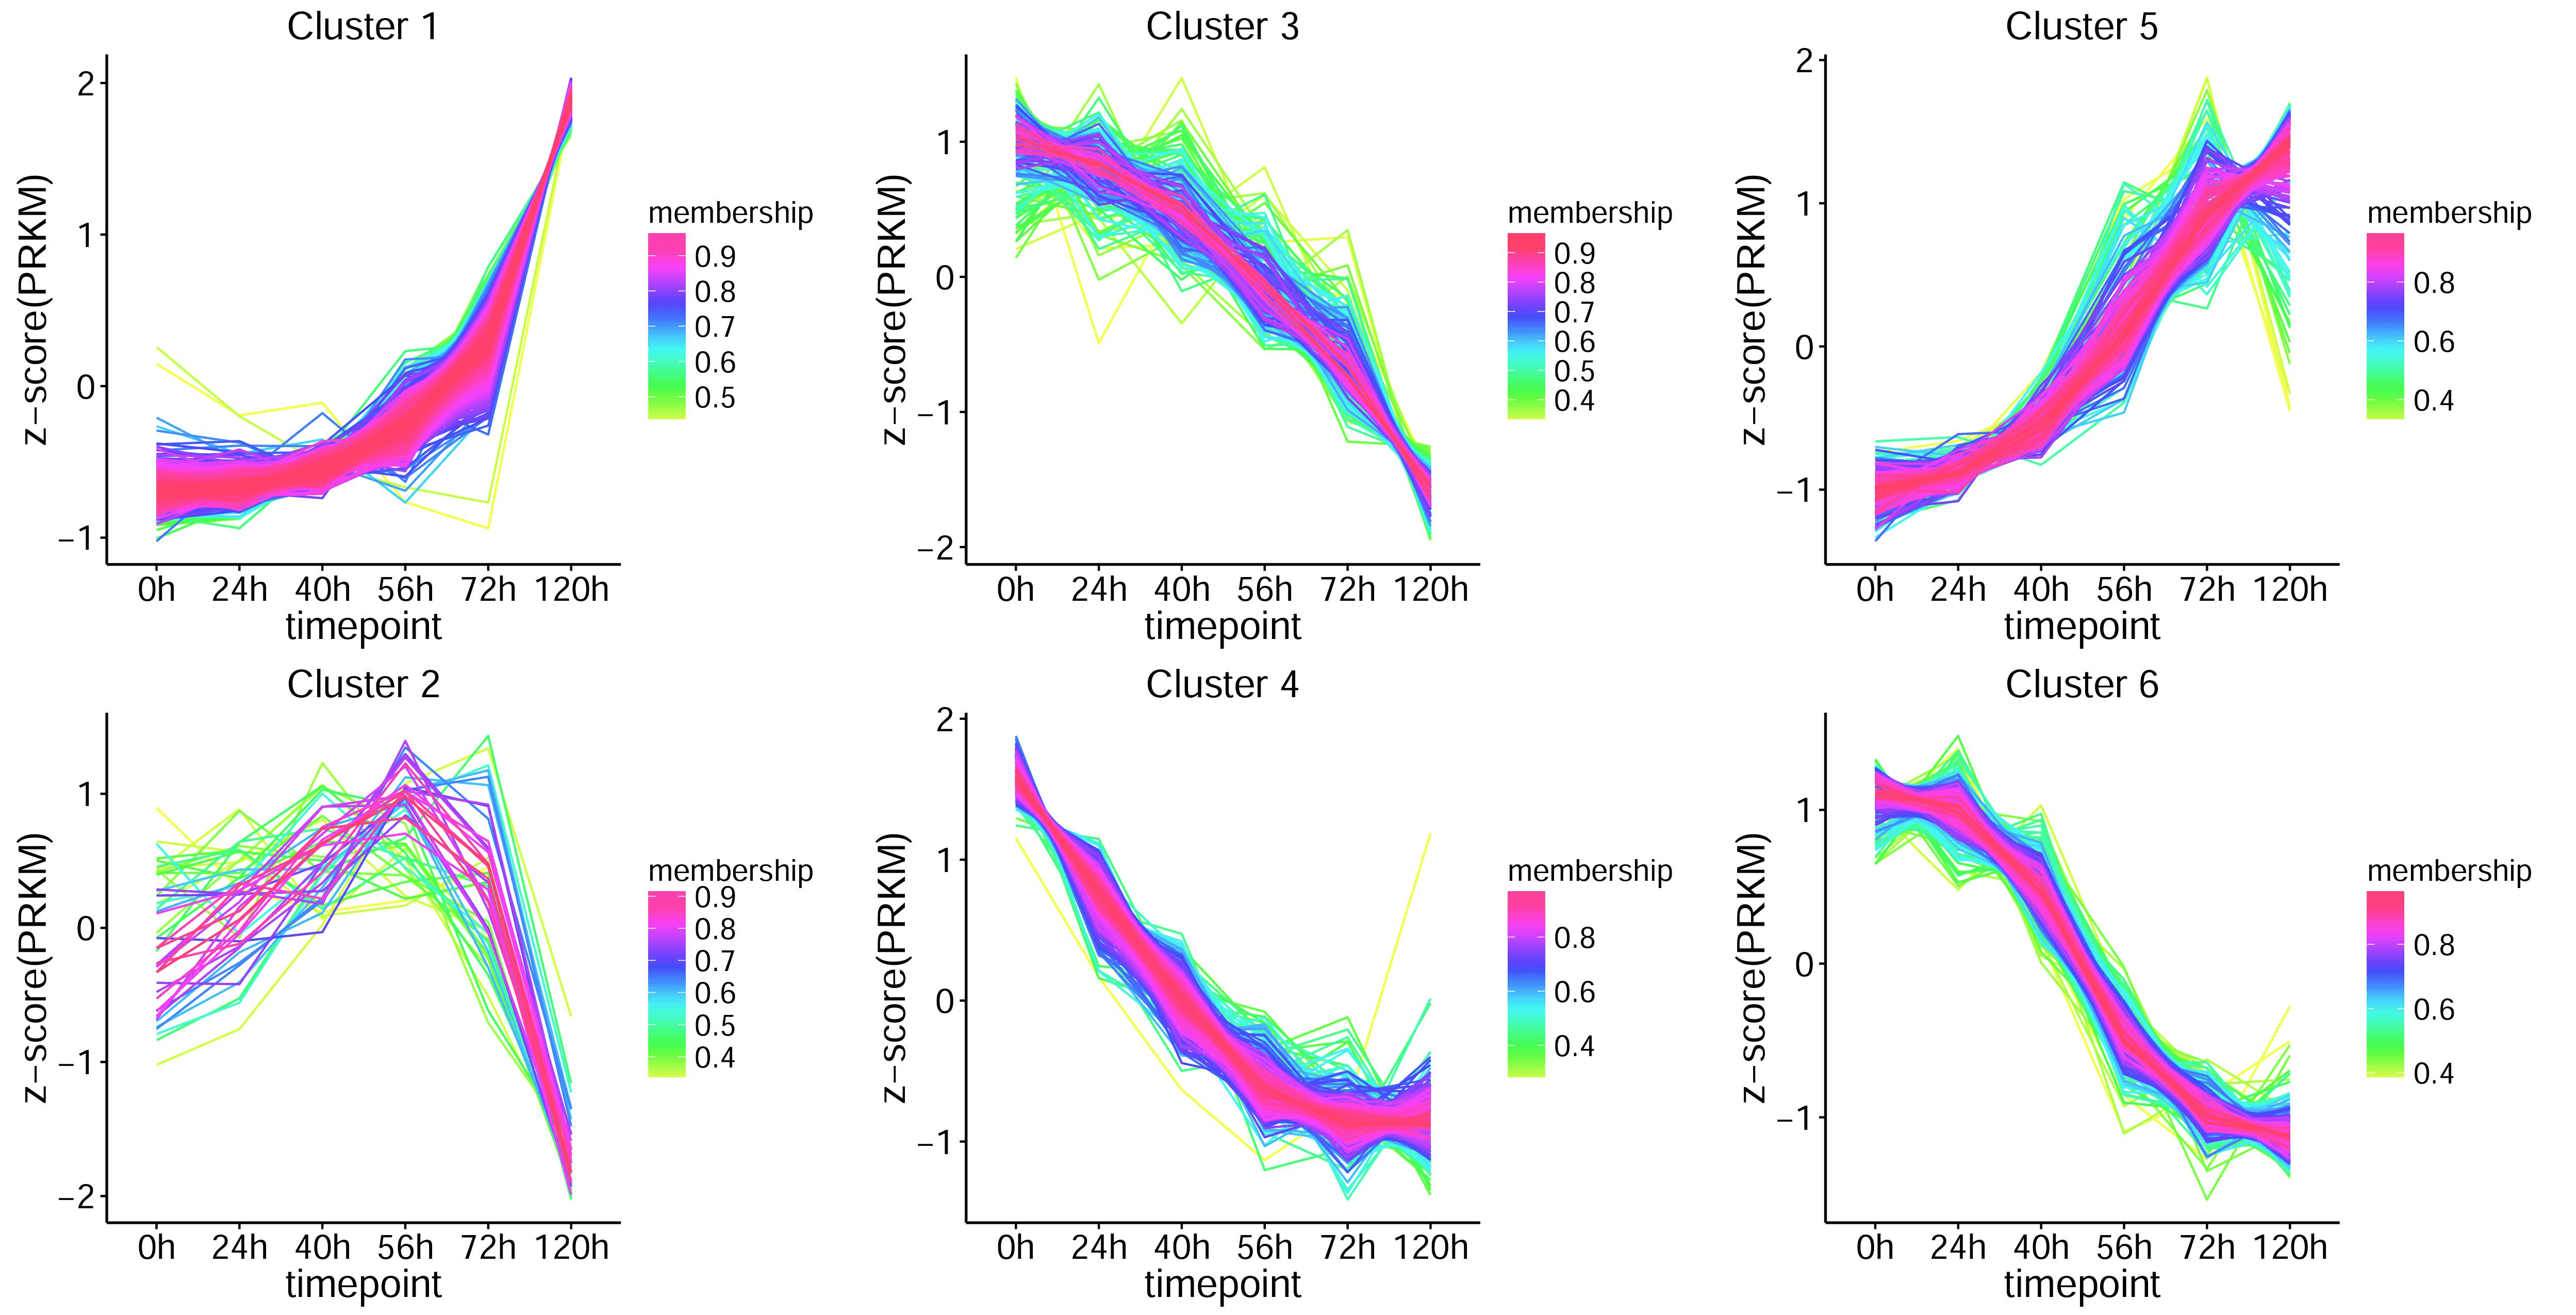
\includegraphics[width=\textwidth]{clusterRes.png}
    \caption{Visualization of clustering results}
\end{figure}

Individual clusters can also be plotted:
\begin{Schunk}
\begin{Sinput}
> #plot cluster 1:
> print(p[[1]])
\end{Sinput}
\end{Schunk}
\begin{figure}[H]
\centering
        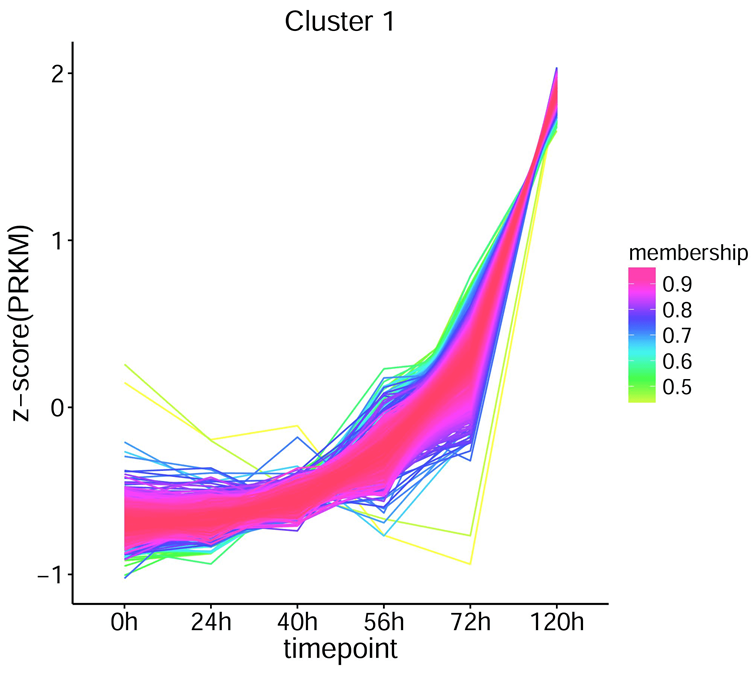
\includegraphics[width=0.5\textwidth]{subcluster.png}
    \caption{Visualization of cluster 1}
\end{figure}

To plot the cmeans clustering results, the TCseq provides several color schemes to color code the membership values which indicate the degree to which data points belong to a cluster.
%--------------------------------------------------
%BIBLIOGRAPHY

\begin{thebibliography}{9}
\bibitem {Robinson} Robinson, M.D., McCarthy, D.J. and Smyth, G.K. edgeR: a Bioconductor package for differential expression analysis of digital gene expression data, Bioinformatics, 26, 139-140,2010.
\bibitem {McCarthy} McCarthy,D.J.,Chen, Y., Smyth, G. K. Differential expression analysis of multifactor RNA-Seq experiments with respect to biological variation. Nucleic acids research 40, 4288-4297,2012.
\bibitem{Futschik} Futschik, M.E. and Carlisle, B. Noise-robust soft clustering of gene expression time-course data, Journal of bioinformatics and computational biology, 3, 965-988, 2005.
\bibitem{lokesh} L. Kumar and M. Futschik, Mfuzz: a software package for soft clustering of microarray data, Bioinformation, 2(1),5-7,2007

\end{thebibliography}

\end{document}
